\documentclass[11pt,twocolumn]{article}

\usepackage{amsmath}
\usepackage{amssymb}
\usepackage{booktabs}
\usepackage{fancyhdr}
\usepackage[includehead,margin=0.5in]{geometry}
\usepackage{graphicx}
\usepackage{helvet}
\usepackage{parskip}  % disable paragraph indent
\usepackage{sectsty}  % change section header formatting

% helvet font settings
\renewcommand{\familydefault}{\sfdefault}

% make figure caption use "Fig."
\makeatletter
\renewcommand{\fnum@figure}{Fig \thefigure}
\makeatother

% make section headers 11 pt font
\sectionfont{\fontsize{11}{15}\selectfont}

\title{\normalsize\textbf{
  FAST SYMBOLIC METHODS FOR MUSCLE-DRIVEN OPTIMAL CONTROL
}}
\author{
Jason K. Moore\textsuperscript{1} and
Samuel G. Brockie\textsuperscript{2} and
Timótheüs J. Stienstra\textsuperscript{3} and
Antonie van den Bogert\textsuperscript{4} \\
\\
% TODO : Make affliations 10pt
\textsuperscript{1}Department of BioMechanical Engineering, Delft University of Technology, The Netherlands\\
\textsuperscript{2}Department of Engineering, University of Cambridge, United Kingdom\\
\textsuperscript{3}Aerospace Engineering, Delft University of Technology, The Netherlands\\
\textsuperscript{4}Mechanical Engineering, Cleveland State University, USA\\
Email: j.k.moore@tudelft.nl}
\date{}

\renewcommand{\thispagestyle}[1]{} % do nothing
\renewcommand{\headrulewidth}{0pt}

\begin{document}
\pagestyle{fancy}
\lhead{}
\rhead{\textbf{XX International Symposium on Computer Simulation in Biomechanics\\
July 23rd – 25th 2025, Uppsala}}
\fancyfoot{}
\maketitle
\section*{INTRODUCTION}
\vspace{-1em}
%
Direct collocation is now widely used for solving biomechanical optimal control
problems. For example, OpenSim includes Moco~\cite{Dembia2019} which allows
users to find optimal control solutions with lower overhead. One advantage of
direct collocation is the speed at which solutions can be found, which can be
orders of magnitude faster than methods which require integrating the
differential equations. Direct collocation methods can still result in overall
slower speed when searching for global minima and choices in the software
design can reduce computational efficiency. For example, Moco relies on finite
differences for gradients which can reduce performance and accuracy.

Solving an optimal control problem resulting from direct collocation requires
evaluating the system's equations of motion, its Jacobian, and possibly its
Hessian thousands to millions of times, but this evaluation is parallelizable
over multiple compute cores and can leverage the massive sparsity of the
equations. Maximizing the compute and memory performance of the functions that
evaluate the constraints and their derivatives allow the subsequent
optimization algorithms to solve very large problems, both in simulation
duration and number of degrees of freedom.

Early dynamics simulation software used computer-aided algebra techniques,
which allowed for analytical derivatives when forming equations of motion, but
this has faded from popularity with the growth of numerical physics engines.
Code generated from computer-aided algebra can be optimized for evaluation
performance using both compiler pre-optimizations and built-in compiler
optimizations that are harder, or even impossible, to apply to numeric physics
engines.

We will demonstrate software that leverages symbolic formulations to generate
computationally efficient parallelized functions based on implicit dynamics to
evaluate the non-linear programming problem's constraints and its derivatives
based on the ideas of \cite{vandenBogert2011a}. We demonstrate solving a 3D
arm-muscle driven bicycle-rider model that has three degrees of freedom and
seven algebraic constraints resulting in millions of floating point operations
in the implicit equations of motion.
%
\begin{table*}[t]
  \centering
  % TODO : Make caption 10pt.
  \caption{Mean performance for the bicycle-rider solution on a Macbook Pro
    with 2.4 GHz 8-Core processor, running Python 3.12.9, SymPy 1.13.3, and
    opty 1.4.0 using Ipopt 3.14.17 with Mumps 5.7.3}
  \scriptsize
  \begin{tabular}{lllllllllll}
    \toprule
    Symbolic &
    Symbolic &
    Constraint &
    Jacobian &
    Symbolic &
    OCP &
    NLP &
    Objective &
    Gradient &
    Constraint &
    Jacobian
    \\
    EoM [s] &
    Jacobian [s] &
    Clang [s] &
    Clang [s] &
    OCP [s] &
    Solve [s] &
    iterations &
    evaluations &
    evaluations &
    evaluations &
    evaluations
    \\
    \midrule
    14.9 &
    35.4 &
    58.3 &
    66.7 &
    169.8 &
    73.0 &
    286 &
    1098 &
    286 &
    1098 &
    292
    \\
    \bottomrule
  \end{tabular}
  \label{tab:performance}
\end{table*}

\vspace{-1em}
\section*{METHODS}
\vspace{-1em}
%
The non-linear equations of motion for musculoskeletal-vehicle system can be
described by differential algebraic equations that are a function of the states
\(\mathbf{y} \in \mathbb{R}^n\), controls \(\mathbf{r}\), and constant
parameters \(\mathbf{p}\), in general. The implicit equations take this form:
%
\begin{align}
  \mathbf{f}(\dot{\mathbf{y}}(t), \mathbf{y}(t), \mathbf{r}(t), \mathbf{p}) =
  \mathbf{0} \in \mathbb{R}^n
\end{align}
%
These equations can contain elements such as musculotendon force-velocity
relationships, kinematic loops, friction and collision forces, etc. We write
these equations as analytically differentiable functions. To map these to
non-linear programming constraints we discretize the equations with backward
Euler differentiation over a constant time step and code generate functions in
C that evaluate the constraints and Jacobian over all \(N\) nodes, while
exploiting the high sparsity of the Jacobian, using opty~\cite{Moore2018}. The
symbolic Jacobian is calculated in forward mode applying the chain rule through
all common sub-expressions which efficiently handles differentiating equations
of motion with many mathematical operations. This results in cacheable
computationally efficient numerical functions that evaluate the non-linear
programming problem constraints and its Jacobian. Evaluation of the objective
is generally a low computational cost, so this is only done in Python, but also
with a symbolic-to-numeric conversion.

To demonstrate our methods, we developed a bicycle-rider model that is the
non-linear Carvallo-Whipple model of the vehicle with four additional rigid
bodies representing the upper and lower arm body segments using
SymBRiM~\cite{Stienstra2023a}. We include four lumped Hill-type muscle models
representing the extensor and flexor groups for the elbow. The model has seven
holonomic constraints and four nonholonomic constraints resulting in a
13\textsuperscript{th} order model with seven algebraic equations. This results
in equations with 2.8M floating point operations in the implicit symbolic
equations of motion. After efficient Jacobian formulation and compiler
pre-optimizations, this reduces to 10K and 69K operations for evaluating the
constraints and Jacobian, respectively. This numerical evaluation time depends
on the number of nodes, so approximately \(N\times\)79K. For \(N=\)~10K we time
the evaluation of these two functions with and without parallelization using
OpenMP 4.5 seeing a 2.5\(\times\) and 2\(\times\) speed up over 64 ms and 500
ms, respectively. Lastly, we define a minimial muscle excitation lane change
tracking task, starting from zero speed up to a mean speed of X m/s over the
fixed duration of X seconds, as an optimal control problem.

% 10K nodes on Jason's laptop
% single thread:
% In [2]: %timeit problem.constraints(initial_guess)
% 64 ms ± 4.21 ms per loop (mean ± std. dev. of 7 runs, 10 loops each)
% In [3]: %timeit problem.jacobian(initial_guess)
% 500 ms ± 44.6 ms per loop (mean ± std. dev. of 7 runs, 1 loop each)
% parallel:
% In [3]: %timeit problem.constraints(initial_guess)
% 25 ms ± 3.36 ms per loop (mean ± std. dev. of 7 runs, 10 loops each)
% In [4]: %timeit problem.jacobian(initial_guess)
% 253 ms ± 38.8 ms per loop (mean ± std. dev. of 7 runs, 1 loop each)

\vspace{-1em}
\section*{RESULTS AND DISCUSSION}
\vspace{-1em}
%
\begin{figure}
    \centering
    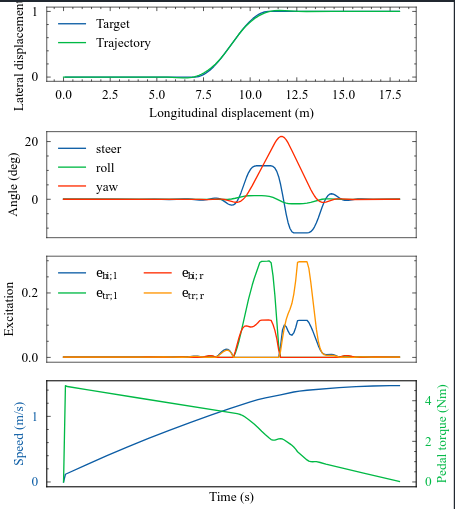
\includegraphics[width=\linewidth]{figures/arm-muscle-bicycle-excitation.png}
    % TODO : Make caption 10pt.
    \caption{Triceps and biceps muscle group excitations for the left and right
      arms to execute a lane change maneuver.}
    \label{fig:trajectories}
\end{figure}

Table~\ref{tab:performance} shows timings for solving an 200 node bicycle-rider
problem. Building the model and forming the optimal control problem takes 185
seconds with most time spent compiling the generated functions with Clang. This
can be cached to disk and need not be built again unless the dynamics model
changes. Ipopt solves the problem to an acceptable level in 73 seconds.
Fig.~\ref{fig:trajectories} shows an example optimal solution.

\vspace{-1em}
\section*{CONCLUSIONS}
\vspace{-1em}
%
Our methods focus on maximizing the performance of evaluating the constraint
and Jacobian numerical functions. The performance of these functions scale
linearly with the number of collocation nodes and can be sped up
multiplicatively by the number of compute cores available. Whenever Ipopt needs
to evaluate these functions thousands or millions of times, for example in a
long duration problem, the overall solution can be minimized.

\vspace{-1em}
% TODO : Change "References" header to all caps
\bibliographystyle{abbrv}
\bibliography{references}

\vspace{-1em}
\section*{ACKNOWLEDGMENTS}
\vspace{-1em}
%
Peter Stahlecker made contributions to the work.

\end{document}
